To maintain a modular and scalable UI, SeatGen’s frontend follows a structured component-based architecture using React. Each UI section, including the map, toolbar, menus, and detail editor, is encapsulated in independent components. These components communicate through React’s state management system and the MapContext to ensure that UI updates remain efficient and consistent.

\begin{figure}[H]
    \begin{center}
        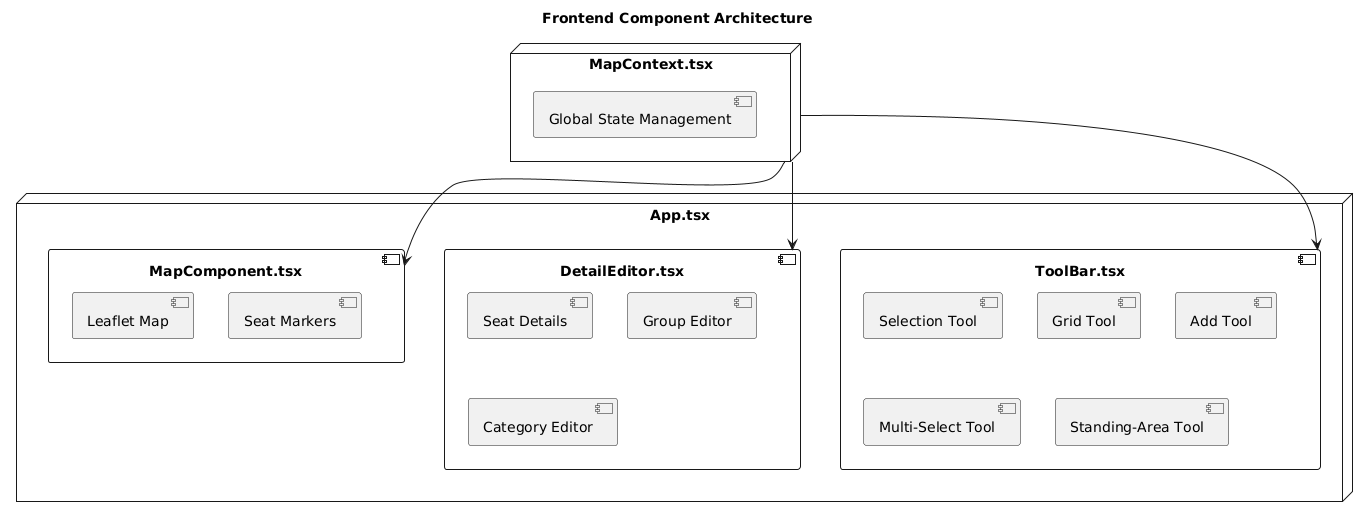
\includegraphics[scale=0.3]{pics/frontend_architecture.png}
    \end{center}
    \caption{Frontend Component Architecture Overview (Rough Overview)}
    \label{fig:frontend-architecture}
\end{figure}

The diagram in Figure~\ref{fig:frontend-architecture} illustrates the core interactive components of the SeatGen frontend. However, it does not represent all UI elements, such as the menu, landing page, modals, and settings, which are also essential for the overall user experience.

Beyond the primary seating map, detail editor, and tool system, SeatGen's frontend also includes:

\begin{itemize}
    \item \textbf{Landing Page (LandingPage.tsx)}: The first screen that users see upon opening SeatGen. It provides an introduction to the tool and a project overview for first-time users.
    
    \item \textbf{Home Menu (Home.tsx)}: This serves as the main project selection interface. Users can choose between loading an already saved seating plan or creating a new one. The UI provides an intuitive and minimalistic selection process while ensuring users can access their projects quickly.
    
    \item \textbf{Menu and Navigation (Menu.tsx)}: The global navigation system connects different views within SeatGen. It allows users to switch between the seating map editor, settings, and export functionalities. The navigation is designed to remain persistent throughout the application to provide seamless transitions between different tasks.
    
    \item \textbf{Settings Panel (SettingsPanel.tsx)}: This panel allows users to configure global preferences that influence the overall seating arrangement experience. Options include:
    \begin{itemize}
        \item \textbf{Default seat categories}: Users can predefine categories to streamline seat assignments.
        \item \textbf{Theme selection}: Dark or light mode based on user preference.
        \item \textbf{Seat map scaling}: Allows fine-tuned adjustments of grid seat density.
    \end{itemize}
    
    \item \textbf{Modals and Popups}: The frontend includes various popups and confirmation dialogs:
    \begin{itemize}
        \item \textbf{Modal.tsx}: Used for confirmations, warnings, and additional actions.
        \item \textbf{LeavePagePopup.tsx}: Warns users about unsaved changes before leaving.
    \end{itemize}
\end{itemize}

These elements, though not included in the diagram, play a significant role in navigating and managing seat plans efficiently and further improving the user experience.


\subsection{MapComponent.tsx: Interactive Map Rendering}
\setauthor{Michael Ruep}
The map is one of the most important components in SeatGen, responsible for rendering and managing the stadium seating map. It integrates with Leaflet library to provide interactive seat visualization, selection, and manipulation.

\subsubsection{Key Responsibilities:}
\begin{itemize}
    \item Initializes and manages the \textbf{Leaflet map instance}.
    \item Loads seat and standing area data dynamically from the backend.
    \item Renders seats and standing areas as \textbf{interactive markers and polygons}.
    \item Handles user interactions such as \textbf{clicking, selecting, and dragging seats}.
    \item Implements \textbf{state synchronization} with the global context (map context).
    \item Provides support for \textbf{tool-based seat editing} (e.g., adding, deleting, moving).
\end{itemize}

\textbf{Component Structure:}
\begin{itemize}
    \item \textbf{State Management:} Uses \texttt{useState}, \texttt{useEffect}, and \texttt{useContext} to manage map data.
    \item \textbf{Leaflet Integration:} Utilizes \texttt{MapContainer} from \texttt{react-leaflet} for seamless map rendering.
    \item \textbf{Performance Enhancements:} Implements \texttt{useCallback} and \texttt{useRef} to optimize re-renders.
\end{itemize}

\subsubsection{Map Initialization and Leaflet Integration}

The map component initializes the Leaflet map using the react-leaflet \texttt{MapContainer} component.

\begin{lstlisting}[language=TypeScript, caption=Initializing Leaflet Map in React, label=lst:react-leaflet]
const MapComponent: FC<MapProps> = ({ editable: initialEditable }) => {
    const context = useMapContext(); // Access global state (MapContext)
    const { bucketName, mapName } = useParams(); // Retrieve map identifiers from URL params

    const [editable, setEditable] = useState(initialEditable ?? true);
    const mapRef = useRef<L.Map>(null);

    return (
        <MapContainer
            crs={L.CRS.Simple} // Uses a flat, pixel-based coordinate system
            className="leaflet-container h-full w-full"
            ref={mapRef}
            center={[context.mapInfo.tileSize / (-2), context.mapInfo.tileSize / (2)]}
            zoom={context.mapInfo.defaultZoom}
            maxZoom={context.mapInfo.maxZoom}
            minZoom={context.mapInfo.minZoom}
            scrollWheelZoom={true}
            zoomControl={false}
            doubleClickZoom={false}
            preferCanvas={true}
            dragging={true}
            tap={false}
            renderer={L.canvas()} // Use Canvas for better performance
        >
            <TileLayer tms={true} url={`${context.mapInfo.mapDto.baseUrl}/{z}/{x}/{y}.png`} />
        </MapContainer>
    );
};
\end{lstlisting}

\textbf{Custom CRS (Coordinate Reference System):}
\begin{itemize}
    \item Uses \textbf{L.CRS.Simple}, a \textbf{2D pixel-based coordinate system}.
    \item Unlike traditional geographic maps, SeatGen does not need a curved map.
    \item All coordinates can be converted to a Cartesian X/Y grid.
\end{itemize}

\textbf{Custom Rendering Engine:}
\begin{itemize}
    \item Uses \textbf{L.canvas()} instead of SVG for performance.
    \item Enables handling of thousands of seat markers.
    \item Reduces DOM load by rendering elements in a drawing surface.
\end{itemize}

\textbf{Dynamically Loading Map Tiles:}
\begin{itemize}
    \item The tile URL is dynamically constructed based on \texttt{context.mapInfo}.
    \item Tiles are loaded asynchronously to improve map load times.
\end{itemize}


\subsubsection{Fetching Seat and Standing Area Data}
\setauthor{Michael Ruep}

The map component fetches seat and standing area data from the backend when the component mounts. This is done using the API client in the \texttt{useEffect} hook.

\begin{lstlisting}[language=TypeScript, caption=Fetching Seat and Category Data, label=lst:fetch-seats]
useEffect(() => {
    if (bucketName && mapName) {
        // Fetch basic stadium map information
        seatgenApiClient.api.info(bucketName, mapName)
            .then(response => context.setMapInfo(response.data))
            .catch(error => console.error('Error fetching map info:', error));

        // Fetch seat categories before retrieving individual seats
        seatgenApiClient.api.getAllCategories().then((r) => {
            if (r.ok) {
                context.setCategories(r.data);
                seatgenApiClient.api.getSeatsByMap(bucketName, mapName).then(response => {
                    if (r.ok) {
                        context.setSeats(response.data.map((s) => ({
                            id: s.seatId!,
                            position: { lat: s.xcoord!, lng: s.ycoord! },
                            category: r.data.find(it => it.id === s.categoryId) ?? null
                        })));
                    }
                });
            }
        });

        // Fetch standing areas
        seatgenApiClient.api.getSectorByMap(bucketName, mapName).then((r) => {
            if (r.ok) {
                context.setStandingAreas(r.data.map((data) => ({
                    id: data.id!,
                    name: data.name!,
                    capacity: data.capacity,
                    coordinates: data.coordinates?.map((c) => new L.LatLng(c.x!, c.y!)) ?? [],
                    selected: false
                })));
            }
        });

    } else {
        console.error("BucketName or MapName not set");
    }
}, [bucketName, mapName]);
\end{lstlisting}

\textbf{Breakdown of Logic:}
\begin{itemize}
    \item Fetches stadium metadata (mapInfo) and sets it globally.
    \item Retrieves seat categories.
    \item Retrieves seat positions from the backend and maps them into React state.
    \item Ensures data consistency by linking seats to their corresponding categories.
\end{itemize}

\textbf{Example of Mapped Seat Object:}
\begin{lstlisting}[language=TypeScript, caption=Seat Object in State, label=lst:seat-object]
{
    id: 1234,
    position: { lat: 48.3069, lng: 14.2858 }, // Example coordinates
    category: { id: 2, name: "VIP", color: "#FFD700" } // Associated category
}
\end{lstlisting}

\subsubsection{Fetching Standing Area / Sector Data}
In addition to seats, the component also retrieves standing areas, which are handled separately.

\begin{lstlisting}[language=TypeScript, caption=Fetching Standing Areas, label=lst:fetch-standingareas]
seatgenApiClient.api.getSectorByMap(bucketName, mapName).then((r) => {
    if (r.ok) {
        context.setStandingAreas(r.data.map((data) => ({
            id: data.id!,
            name: data.name!,
            capacity: data.capacity,
            coordinates: data.coordinates?.map((c) => new L.LatLng(c.x!, c.y!)) ?? [],
            selected: false
        })));
    }
});
\end{lstlisting}

\textbf{Explanation:}
\begin{itemize}
    \item The API returns a list of sector polygons.
    \item Each area consists of a unique id, name, capacity, and a list of coordinates.
    \item Coordinates are transformed into Leaflet’s LatLng format to be rendered as a polygon.
\end{itemize}

\textbf{Example of a Standing Area Object in State:}
\begin{lstlisting}[language=TypeScript, caption=Standing Area Object in State, label=lst:standingarea-object]
{
    id: 69420,
    name: "Sektor 69",
    capacity: 187,
    coordinates: [
        { lat: 48.3069, lng: 14.2858 },
        { lat: 48.3075, lng: 14.2862 },
        { lat: 48.3080, lng: 14.2856 }
    ],
    selected: false
}
\end{lstlisting}

\subsubsection{State Management and Performance}
\begin{itemize}
    \item \texttt{useEffect} Dependency Array:
    \begin{itemize}
        \item Ensures the API calls only run when \texttt{bucketName} or \texttt{mapName} change.
        \item Prevents unnecessary re-fetching on every render.
    \end{itemize}
    
    \item Efficient State Updates:
    \begin{itemize}
        \item Avoids unnecessary re-renders by batching state updates for seats and standing areas.
        \item No prop-drilling by storing fetched data needed globally in the map context.
    \end{itemize}

    \item Error Handling:
    \begin{itemize}
        \item If any API call fails, an error is logged, and the operation is skipped.
        \item Ensures that failures in one request do not crash the entire component.
    \end{itemize}
\end{itemize}

\subsubsection{Rendering Seats and Handling Selection}
\setauthor{Michael Ruep}

Each seat in the stadium is rendered as a Leaflet marker, allowing users to interact with them dynamically. The selection mechanism is designed to provide an intuitive experience while supporting multi-selection for bulk operations.

\textbf{Rendering Seat Markers:}
\begin{lstlisting}[language=TypeScript, caption=Rendering and Selecting Seats, label=lst:seat-rendering]
const handleSeatClick = useCallback((id: number, event: L.LeafletMouseEvent) => {
    const isCtrlPressed = event.originalEvent?.ctrlKey;

    context.setSeats(prevSeats => prevSeats.map(seat => {
        if (seat.id === id) {
            const selected = isCtrlPressed ? !seat.selected : true;
            return { ...seat, selected };
        }
        return isCtrlPressed ? seat : { ...seat, selected: false };
    }));

    setOpenSideBar(true);
}, [context]);
\end{lstlisting}

\textbf{How This Works:}
\begin{itemize}
    \item Clicking a seat toggles its selected state.
    \item Holding \texttt{Ctrl} allows multi-selection, useful for bulk actions.
    \item Clicking a seat opens the detail editor sidebar for further modifications.
\end{itemize}


\subsubsection{Implementing Live Seat Dragging and Moving}
\setauthor{Michael Ruep}

In SeatGen, users can drag and reposition multiple selected seats dynamically. The challenge was ensuring that \textbf{all} selected seats move smoothly and live directly following the cursor while keeping their relative distances intact. To achieve this, a real-time position tracking mechanism was implemented using Leaflet events and React state updates.

\subsubsection{Tracking Initial Positions}
Before moving seats, their initial positions are stored so that relative offsets can be preserved:

\begin{lstlisting}[language=TypeScript, caption=Storing Initial Positions Before Dragging, label=lst:seat-initial-pos]
const initialPositionsRef = useRef<{ [key: number]: L.Point }>({});

const storeInitialPositions = useCallback(() => {
    const map = mapRef.current;
    if (!map) return;

    initialPositionsRef.current = {};
    selectedSeats.forEach(seat => {
        initialPositionsRef.current[seat.id] = map.latLngToLayerPoint(seat.position);
    });

    // Register move action for undo functionality
    context.doAction(new MoveAction(selectedSeats, context.setSeats));
}, [selectedSeats, context]);
\end{lstlisting}

\textbf{How This Works:}
\begin{itemize}
    \item A reference (\texttt{initialPositionsRef}) is created to store the pixel positions of selected seats by converting the Latitude and Longitude into Layer Points which are x and y Cartesian System points.
    \item These positions are saved when the user starts dragging a seat.
    \item The relative distance between seats is maintained, preventing unwanted misalignment.
\end{itemize}

\subsubsection{Updating Seats in Real-Time During Dragging}
While the user drags a seat, the drag distance is calculated and applied to all selected seats:

\begin{lstlisting}[language=TypeScript, caption=Updating Seat Positions During Dragging, label=lst:seat-live-dragging]
const updateSelectedSeatsPosition = useCallback((draggedSeatId: number, newLatLngPosition: { lat: number; lng: number }) => {
    const map = mapRef.current;
    const primarySeat = context.seats.find(s => s.id === draggedSeatId);

    if (!map || !primarySeat || !primarySeat.selected) return;

    const newPosition = map.latLngToLayerPoint(newLatLngPosition);
    const oldPosition = initialPositionsRef.current[draggedSeatId];

    const deltaX = newPosition.x - oldPosition.x;
    const deltaY = newPosition.y - oldPosition.y;

    context.setSeats(prevSeats =>
        prevSeats.map(seat => {
            if (seat.selected) {
                const initialPosition = initialPositionsRef.current[seat.id];
                const newPosX = initialPosition.x + deltaX;
                const newPosY = initialPosition.y + deltaY;
                const newLatLngPos = map.layerPointToLatLng(new L.Point(newPosX, newPosY));
                return { ...seat, position: newLatLngPos };
            }
            return seat;
        })
    );

    // Update MoveAction for undo tracking
    const currentAction = context.getCurrentAction();
    if (currentAction instanceof MoveAction) {
        currentAction.setNewSeats(selectedSeats);
    }
}, [context.seats, context]);
\end{lstlisting}

\textbf{Breakdown of Logic:}
\begin{itemize}
    \item The drag delta (change in X/Y position) between the starting position and the new cursor position is calculated.
    \item The same delta is applied to all selected seats, ensuring they move together.
    \item Positions are converted between LatLng (geo-coordinates) and pixel points, so dragging works consistently at different zoom levels.
    \item Changes using \texttt{MoveAction} are tracked, allowing the operation to be undone if needed.
\end{itemize}

\subsubsection{Optimizations and Challenges}
\textbf{Major Challenges Encountered:}
\begin{itemize}
    \item Preventing position drift when switching between zoom levels.
    \item Ensuring smooth movement with large seat selections.
    \item Avoiding excessive re-renders that slow down performance.
\end{itemize}

\textbf{Performance Optimizations:}
\begin{itemize}
    \item Used \texttt{useRef} to store initial positions instead of state (prevents extra re-renders).
    \item Applied batch updates for all selected seats instead of updating them individually.
    \item Optimized Leaflet latLng-to-pixel conversion to enable natural seat dragging (direct manipulation \cite{Hutchins01121985}).
\end{itemize}

\subsubsection{Conclusion}
The live dragging implementation allows users to dynamically reposition multiple seats while keeping their relative distances intact. By leveraging Leaflet’s coordinate system and real-time state updates, a fluid and high-performance dragging experience was achieved, with full undo and redo functionality.

\subsubsection{Managing Standing Areas and Sectors}
\setauthor{Michael Ruep}

SeatGen allows the definition of standing areas / sectors, which differ from regular seats by not being assigned individual markers but instead represented as polygonal sectors. Each standing area has a defined capacity, ensuring ticketing restrictions.

\textbf{Standing Area Features:}
\begin{itemize}
    \item \textbf{Custom Polygons:} Users define standing areas by selecting points on the map.
    \item \textbf{Capacity Control:} Limits the number of tickets available per standing area.
    \item \textbf{Category Assignment:} Standing areas can be assigned different categories.
    \item \textbf{Real-time Editing:} Areas can be renamed, and deleted dynamically.
\end{itemize}

\textbf{Standing Area Selection:}
\begin{lstlisting}[language=TypeScript, caption=Handling Standing Area Selection, label=lst:select-standingareas]
const handlePolygonClick = useCallback((id: number, event: L.LeafletMouseEvent) => {
    const isCtrlPressed = event.originalEvent?.ctrlKey;

    // Deselect all seats when a polygon is clicked
    context.setSeats(prevSeats => prevSeats.map(seat => ({
        ...seat,
        selected: false
    })));

    const selectedStandingAreaIds: number[] = [];
    context.setStandingAreas(prevAreas => {
        return prevAreas.map(area => {
            if (area.id === id) {
                const selected = isCtrlPressed ? !area.selected : true;
                if (selected) selectedStandingAreaIds.push(area.id);
                return { ...area, selected };
            }
            if (!isCtrlPressed) {
                return { ...area, selected: false };
            }
            if (area.selected) selectedStandingAreaIds.push(area.id);
            return area;
        });
    });
    // Update the selected standing area ids in the context
    context.setSelectedStandingAreaIds(selectedStandingAreaIds);
    setOpenSideBar(true);
}, [context, setOpenSideBar]);
\end{lstlisting}

\textbf{Selection and Editing Process:}
\begin{itemize}
    \item Clicking a standing area toggles its selected state.
    \item In the detail editor panel, renaming, capacity adjustments, and category (including color coding) updates are possible.
\end{itemize}

\begin{figure}[H]
    \centering
    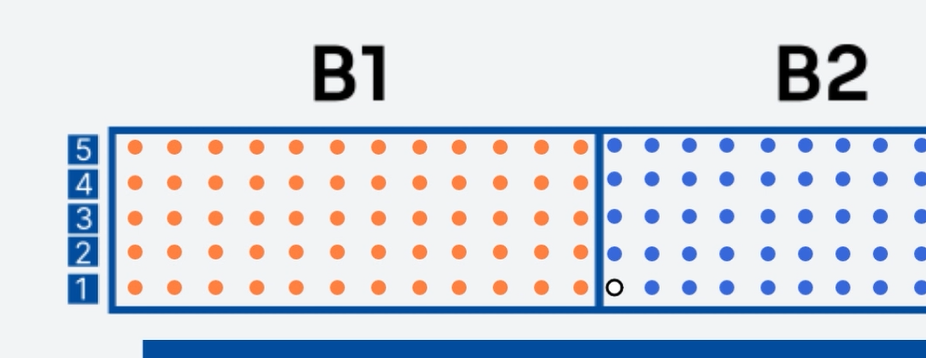
\includegraphics[width=0.7\textwidth]{pics/MapComponentCategoryAndSelectedSeat.png}
    \caption{Seats with Category Color, and Selected Seat}
    \label{fig:map-component-category}
\end{figure}

\subsubsection{Event Handling in Leaflet}
\setauthor{Michael Ruep}

SeatGen relies heavily on Leaflet event handling to manage user interactions dynamically. TODO Deselection
TODO Drag Events for Seat Movement + reference

\begin{lstlisting}[language=TypeScript, caption=Handling Seat Drag Events, label=lst:leaflet-seat-drag]
// Function definitions for handling drag events
const handleDragStart = (seatId: number) => {
    storeInitialPositions();
};

const handleDragEnd = (seatId: number, newPosition: L.LatLng) => {
    updateSelectedSeatsPosition(seatId, newPosition);
};

// Applying event listeners to each seat marker
const renderedSeats = useMemo(() => {
    return context.seats.map(seat => (
        <Seat 
            key={seat.id} 
            id={seat.id}
            position={seat.position} 
            updatePosition={updateSeatPosition}
            updateSelectedSeatsPosition={updateSelectedSeatsPosition}
            storeInitialPositions={storeInitialPositions} 
            tooltipText={seat.tooltipText}
            onClick={(event: LeafletMouseEvent) => handleSeatClick(seat.id, event)}
            onDragStart={() => handleDragStart(seat.id)}
            onDragEnd={(event) => handleDragEnd(seat.id, event.target.getLatLng())}
            draggable={editable}
            selected={seat.selected}
            category={seat.category}
        />
    ));
}, [context.seats, selectedSeats]);
\end{lstlisting}

\begin{itemize}
    \item The handleDragStart function is called when a user begins dragging a seat. It stores the initial positions of selected seats to ensure relative movement.
    \item The handleDragEnd function finalizes the new seat positions when dragging stops.
    \item Event listeners (onDragStart and onDragEnd) are added to each Seat component to trigger these functions dynamically.
    \item The useMemo hook optimizes rendering performance by ensuring seat markers are not unnecessarily re-created during re-renders.
\end{itemize}

\subsubsection{Saving and Syncing with the Backend}
\setauthor{Michael Ruep}
SeatGen implements an asynchronous saving mechanism that synchronizes data with the backend.

TODO: Batch save name, Flow

\textbf{Batch Save:}
\begin{lstlisting}[language=TypeScript, caption=Batch Save Mechanism, label=lst:batch-save-seats]
const saveChanges = useCallback(() => {
    seatgenApiClient.api.saveSeats(bucketName, mapName, context.seats.map(seat => ({
        id: seat.id,
        x: seat.position.lat,
        y: seat.position.lng,
        categoryId: seat.category?.id
    })))
    .then(() => enqueueSnackbar("Changes saved successfully!", { variant: "success" }));
}, [context.seats]);
\end{lstlisting}

\textbf{Batch Save Mechanism:}
\begin{itemize}
    \item Instead of saving each individual seat change separately, SeatGen groups multiple seat updates into a single API request to reduce network overhead and improve efficiency.
    \item The \texttt{useCallback} hook ensures that changes get only saved when \texttt{context.seats} changes, preventing redundant function executions.
    \item \texttt{seatgenApiClient.api.saveSeats} sends the updated seat data to the backend, including the seat id, coordinates, and category id.
    \item Upon a successful save, a snackbar notification is displayed to confirm the operation.
    \item SeatGen maintains the action history so users can revert unintended changes before saving.
\end{itemize}

This saving mechanism ensures that the application remains responsive while keeping data integrity intact, even in scenarios where users forget to manually save their progress, they will be reminded.

\subsubsection{Summary}
The map is the core of SeatGen’s interactive seating system. It efficiently manages:
\begin{itemize}
    \item Interactive Leaflet-based Map Rendering
    \item Seat and Standing Area Rendering
    \item Group Selection and Bulk Editing
    \item Drag-and-Drop Seat Repositioning
    \item Event Handling for User Interaction
    \item Synchronizing data with global state (map context)
    \item Asynchronous Backend Synchronization
\end{itemize}

It ensures smooth operation even for large stadium layouts with thousands of seats.



\subsection{DetailEditor.tsx: Editing Attributes}
\setauthor{Michael Ruep}
The \textbf{DetailEditor.tsx} component provides an interface for modifying selected seats, managing seat groups, categories, and configuring standing areas. It plays a huge role in SeatGen’s user interaction system by allowing users to efficiently modify stadium layouts in a structured and intuitive manner.

\textbf{Key Responsibilities:}
\begin{itemize}
    \item \textbf{Editing Individual Seats:} Users can update seat tooltips, positions, and categories.
    \item \textbf{Managing Seat Groups:} Enables users to create, merge, and delete groups of seats.
    \item \textbf{Standing Area Editing:} Supports renaming and capacity adjustments for standing areas.
    \item \textbf{Category Assignment:} Allows users to assign pricing tiers and colors to seats.
\end{itemize}

\subsection{Component Structure}
The \textbf{DetailEditor.tsx} has the following core sections:
\begin{itemize}
    \item \textbf{Seat Editing Panel:} Displays detailed information for selected seats and allows modifications.
    \item \textbf{Group Management Panel:} Handles seat grouping and bulk operations.
    \item \textbf{Standing Area Editing Panel:} Enables editing of standing areas, including name and capacity.
    \item \textbf{Deletion and Bulk Actions:} Supports removing selected seats, groups, or selected standing areas.
\end{itemize}

\begin{figure}[H]
    \centering
    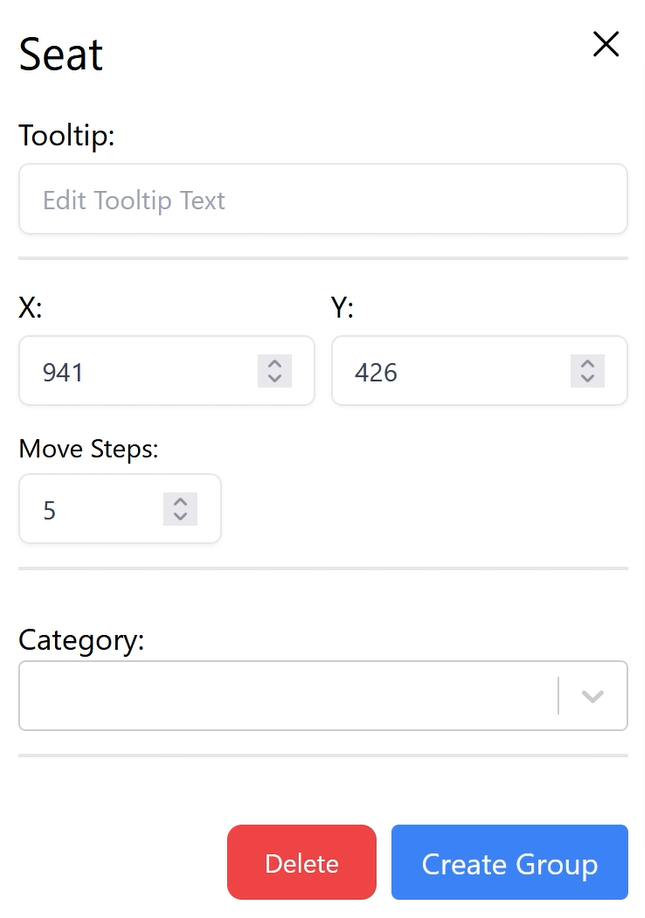
\includegraphics[width=0.6\textwidth]{pics/DetailEditorSeat.png}
    \caption{Seat Editing Panel in DetailEditor.tsx}
    \label{fig:detail-editor-seat}
\end{figure}

Figure~\ref{fig:detail-editor-seat} illustrates the seat editing panel, where users can adjust tooltips, assign categories, and delete seats.

\subsection{Managing Seat Attributes}
When a seat is selected, the editor provides multiple options for modification.

\subsubsection{Updating Tooltip Text}
Users can edit tooltip descriptions for seats, making it easier to add position information or other special notes.

\begin{lstlisting}[language=TypeScript, caption=Updating Tooltip for Selected Seats, label=lst:update-tooltip]
<input
    type="text"
    value={props.currentTooltip}
    onChange={props.handleExternalTooltipChange}
    placeholder="Edit Tooltip Text"
/>
\end{lstlisting}

\textbf{How It Works:}
\begin{itemize}
    \item The text input dynamically updates the tooltip for all selected seats by calling the \texttt{handleExternalTooltipChange} function.
    \item Changes are stored in the global state.
    \item Provides immediate visual feedback to the user.
\end{itemize}

\subsubsection{Adjusting Seat Position via UI}
Instead of manually dragging seats on the map, users can fine-tune their positions numerically. Also, adjusting the steps of one increment when using the arrow keys to position the seats perfectly is possible.

\begin{lstlisting}[language=TypeScript, caption=Updating Seat Coordinates, label=lst:update-seat-position]
const updateSeatPosition = (x: number, y: number) => {
    const latLng = props.mapRef.current!.layerPointToLatLng(new L.Point(x, y));
    props.updateSelectedSeatsPosition(selectedSeats[0].id, { lat: latLng.lat, lng: latLng.lng }, true);
};
\end{lstlisting}

\textbf{How It Works:}
\begin{itemize}
    \item Converts user-inputted X/Y values into map coordinates.
    \item Updates seat position dynamically.
    \item With this the movement is optimized for both manual entry and real-time adjustments.
\end{itemize}

\subsection{Group Management and Multi-Selection}
Grouping seats allows users to efficiently manage large stadium sections.
\subsubsection{Groups and Multi Selection and Deletion}

SeatGen supports the concept of seat groups, allowing users to efficiently manipulate multiple seats at once. Grouping seats enables bulk operations such as movement, category assignment, and section-wide modifications, making it particularly useful for managing large stadium layouts.

\textbf{Use Cases for Seat Groups:}
\begin{itemize}
    \item \textbf{Bulk Editing:} Modify multiple seat attributes simultaneously.
    \item \textbf{Efficient Repositioning:} Move multiple seats while maintaining relative positioning.
    \item \textbf{Category Assignment:} Assign pricing tiers and access restrictions to an entire section.
    \item \textbf{Simplified Deletion:} Remove entire seat groups without manually selecting each seat.
\end{itemize}

\textbf{Creating a Seat Group:}
\begin{lstlisting}[language=TypeScript, caption=Creating Seat Groups, label=lst:create-seat-group]
const createGroup = useCallback(() => {
    context.doAction(new CreateGroupAction(setSeatGroups, selectedSeats));
}, [selectedSeats, context]);
\end{lstlisting}

\textbf{How It Works:}
\begin{itemize}
    \item The function retrieves all currently selected seats.
    \item The CreateGroupAction is executed, registering the selected seats as a group.
    \item The group ID is assigned, and the group is stored in the global state.
\end{itemize}

\textbf{Deleting a Seat Group:}
\begin{lstlisting}[language=TypeScript, caption=Deleting Seat Groups, label=lst:delete-seat-group]
const deleteGroup = useCallback((groupId: number) => {
    context.doAction(new DeleteGroupAction(setSeatGroups, groupId));
}, [context]);
\end{lstlisting}

\textbf{Group Deletion Process:}
\begin{itemize}
    \item The DeleteGroupAction removes all seats within that group using the groupId.
    \item The global context state updates accordingly.
    \item The operation is reversible via the undo stack.
\end{itemize}

Furthermore, users can merge existing groups or split them dynamically, enabling flexible seat management. This allows for unlimited subgrouping, making the editor more intuitive and efficient.

\subsubsection{Seat Categories}
\setauthor{Michael Ruep}

Seat categories allow users to classify seating arrangements based on (pricing) tiers, accessibility, and special designations such as VIP areas or restricted sections. In SeatGen, every seat can be assigned a category that determines its visual representation and ticketing attributes.

\begin{figure}[H]
    \centering
    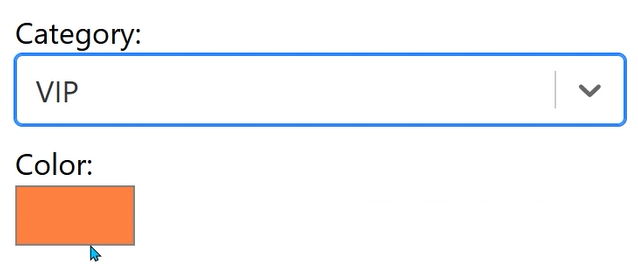
\includegraphics[width=0.7\textwidth]{pics/DetailEditorCategory.png}
    \caption{Category Selection in DetailEditor.tsx}
    \label{fig:detail-editor-category}
\end{figure}

\textbf{Features of Seat Categories:}
\begin{itemize}
    \item \textbf{Color-Coding:} Each category is assigned a color for clear visualization.
    \item \textbf{Pricing Information:} Categories define pricing tiers, ensuring correct ticket pricing.
    \item \textbf{Flexible Assignments:} Seats can be reassigned to different categories as needed.
    \item \textbf{Bulk Category Updates:} Multiple seats can be assigned a category simultaneously.
\end{itemize}

\subsubsection{Category Data Model}

Each seat category is stored as an object that holds classification data:

\begin{lstlisting}[language=TypeScript, caption=Seat Category Data Model, label=lst:seat-category-model]
interface Category {
    id?: number;
    name: string; // Example: "VIP", "General Admission"
    color: string; // Hex code for UI representation
    price: number; // Ticket price associated with this category
}
\end{lstlisting}

\subsubsection{Assigning Categories to Seats}

When a user selects a seat, they can assign or change its category using the \textbf{DetailEditor.tsx}.

\begin{lstlisting}[language=TypeScript, caption=onChange Assigning Categories to Selected Seats, label=lst:assign-category]
onChange={(newVal) => {
    console.log(newVal)
    context.doAction(new UpdateCategoryAction(selectedSeats, newVal ? newVal.value : null))
    setCurrentSelectedCategory(newVal ? newVal.value : null);
}}
\end{lstlisting}

\begin{lstlisting}[language=TypeScript, caption=Assigning Categories to Selected Seats, label=lst:assign-category]
execute = () => {
    this._oldCategories = this._selectedSeats.map(seat => seat.category)
    this._selectedSeats.forEach((seat) => {
        seat.category = this._newCategory
    });
}
\end{lstlisting}

\textbf{How It Works:}
\begin{itemize}
    \item The function in \texttt{UpdateCategoryAction} loops through all selected seats.
    \item The new category is assigned based on the provided \texttt{categoryId}.
    \item The UI updates instantly, applying the new color and classification.
\end{itemize}

\subsubsection{Category Management in the UI}

Users can manage categories by:
\begin{itemize}
    \item Creating new categories with custom colors and pricing.
    \item Editing existing categories, updating names, prices, or colors.
    \item Deleting unused categories.
\end{itemize}

\begin{lstlisting}[language=TypeScript, caption=Managing Categories, label=lst:manage-categories]
onCreateOption={(inputValue) =>
    seatgenApiClient.api.createCategory({name: inputValue, color: "#3768db"}).then((r) => {
        if (r.ok) {
            enqueueSnackbar("Successfully created category", {variant: 'success'})
            selectedSeats.forEach((seat) => {
                seat.category = r.data;
            });
            context.setCategories(prevCategories => [...prevCategories, r.data]);
            context.categoryChecksums.current.set(r.data.id!, objectHash(r.data))
            setCurrentSelectedCategory(r.data)
        } else {
            console.error('Error creating category:', r.statusText);
            enqueueSnackbar('Error creating category', {variant: 'error'});
        }
    })
}
\end{lstlisting}

\begin{lstlisting}[language=TypeScript, caption=Managing Category Color, label=lst:manage-categories]
<input 
    type="color"
    value={currentSelectedCategory.color ?? "#3768db"}
    onChange={(newColor) => {
        selectedSeats[0].category!.color = newColor.target.value
        setCurrentSelectedCategory({...currentSelectedCategory, color: newColor.target.value})
    }));
}}/>
\end{lstlisting}

\subsubsection{Category Visualization on the Map}

Seat categories are visually represented by color-coded markers in \textbf{MapComponent.tsx}. Each seat marker dynamically updates based on its assigned category.

\begin{lstlisting}[language=TypeScript, caption=Rendering Seat Markers with Categories, label=lst:render-seat-category]
const renderedSeats = seats.map(seat => (
    <SeatMarker 
        key={seat.id} 
        seat={seat} 
        color={seat.category?.color || "gray"} 
        onClick={() => handleSeatClick(seat.id)}
    />
));
\end{lstlisting}

\textbf{How It Works:}
\begin{itemize}
    \item Each seat marker inherits the category's color.
    \item Unassigned seats default to a neutral color (gray).
    \item Selecting a seat allows users to change its category.
\end{itemize}

\subsubsection{Conclusion}
Categories play a crucial role in SeatGen, providing a structured way to manage ticket pricing and seat classification. By integrating category assignment with group selection and bulk operations, users can efficiently update stadium layouts with minimal effort.

\subsection{Standing Area Editing}
\setauthor{Michael Ruep}
Standing areas in SeatGen are defined as polygonal sectors rather than individual seats. Unlike seats, which are represented as distinct markers, standing areas are implementd using a defined boundary of polygons. Each standing area has a name, and a maximum capacity.

\textbf{Key Features of Standing Areas:}
\begin{itemize}
    \item \textbf{Custom Polygonal Boundaries:} Users can define standing areas by selecting points on the map.
    \item \textbf{Capacity Control:} Each area has a maximum capacity limit.
    \item \textbf{Real-Time Editing:} Users can rename standing areas and adjust their capacities dynamically.
    \item \textbf{Deletion and Reconfiguration:} Existing standing areas can be removed or modified at any time.
\end{itemize}

\subsubsection{Standing Area Data Model}
Each standing area is stored as an object in the application state.

\begin{lstlisting}[language=TypeScript, caption=Standing Area Data Model, label=lst:standingarea-model]
interface StandingArea {
    id: number;
    name: string; // Display name of the standing area
    capacity: number; // Maximum allowed attendees
    coordinates: L.LatLng[]; // List of boundary points defining the area
    selected: boolean; // Boolean flag indicating selection state
}
\end{lstlisting}

\subsubsection{Creating and Selecting Standing Areas}
Standing areas are created by defining polygonal boundary coordinates on the map. Once an area is selected, it becomes editable in the \texttt{DetailEditor.tsx}.

\subsubsection{Renaming a Standing Area}
Users can rename standing areas directly in the \texttt{DetailEditor.tsx} panel.

\begin{lstlisting}[language=TypeScript, caption=Renaming Standing Areas, label=lst:rename-standingarea]
const handleStandingNameChange = (name: string) => {
    context.setStandingAreas(prev => prev.map(area =>
        context.selectedStandingAreaIds.includes(area.id)
            ? { ...area, name: name }
            : area
    ));
};
\end{lstlisting}

\textbf{How It Works:}
\begin{itemize}
    \item The function updates the name of all selected standing areas.
    \item Changes are reflected instantly in the UI.
    \item The new name is stored persistently for future sessions.
\end{itemize}

\subsubsection{Updating Standing Area Capacity}
To control attendee limits, each standing area has an adjustable capacity.

\begin{lstlisting}[language=TypeScript, caption=Updating Standing Area Capacity, label=lst:update-standingarea-capacity]
const handleStandingCapacityChange = (capacity: string) => {
    context.setStandingAreas(prev => prev.map(area =>
        context.selectedStandingAreaIds.includes(area.id)
            ? { ...area, capacity: Number(capacity) }
            : area
    ));
};
\end{lstlisting}

\textbf{Capacity Adjustment Process:}
\begin{itemize}
    \item The function modifies the capacity of all selected standing areas.
    \item Input validation ensures that only numeric values are accepted.
    \item The UI dynamically updates, reflecting the new ticketing constraints.
\end{itemize}

\subsubsection{Deleting a Standing Area}
Standing areas can be removed using \texttt{DeleteStandingAreaAction} when no longer needed which is also undoable for user convenience.

\begin{lstlisting}[language=TypeScript, caption=Deleting Standing Areas, label=lst:delete-standingarea]
context.doAction(new DeleteStandingAreaAction(selectedStandingAreas, context))

\end{lstlisting}

\begin{figure}[H]
    \centering
    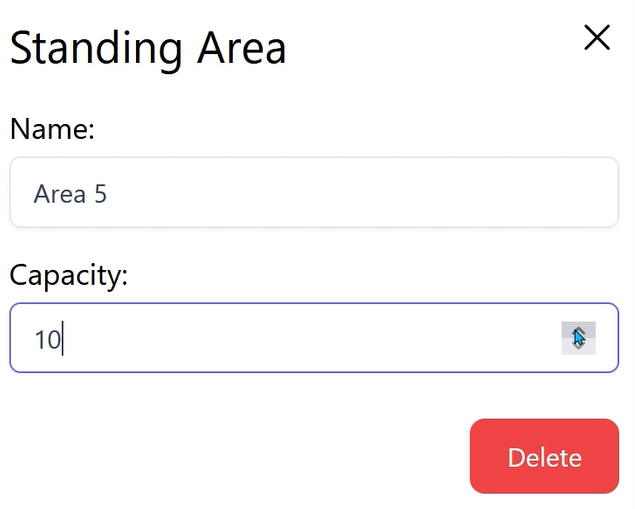
\includegraphics[width=0.7\textwidth]{pics/DetailEditorStandingArea.png}
    \caption{Editing Standing Areas in DetailEditor.tsx}
    \label{fig:detail-editor-standingarea}
\end{figure}

Figure~\ref{fig:detail-editor-standingarea} illustrates the interface for editing standing areas, including renaming, capacity adjustment, and deletion.

Standing areas in SeatGen offer a structured approach to handling non-seated sections of a stadium. By allowing dynamic capacity control and easy renaming, the system ensures that standing areas remain flexible and adaptable. Users can efficiently create, edit, and remove standing areas based on event needs, making stadium layouts highly customizable.

Beyond general standing areas, this feature can also be used to designate specific sections for specialized needs. For example, stadiums may allocate certain sectors for \textbf{wheelchair-accessible areas} or \textbf{priority seating for individuals with mobility impairments}. This flexibility ensures that accessibility requirements can be met while maintaining a clear and organized seating plan.

\subsubsection{Summary}
\textbf{DetailEditor.tsx} is a key component within SeatGen, offering intuitive tools for modifying stadium layouts. It enables:
\begin{itemize}
    \item \textbf{Seat Editing:} Real-time adjustments to tooltips, positions, and assignments.
    \item \textbf{Group Management:} Merging, splitting, and deleting seat groups efficiently.
    \item \textbf{Category Assignment:} Bulk updates with intuitive color-coded visualization.
    \item \textbf{Standing Area Modifications:} Easy editing of boundaries and capacities.
    \item \textbf{Seamless Integration:} Ensures consistent updates via \texttt{MapContext.tsx}.
\end{itemize}

With its structured approach and live updates, \textbf{DetailEditor.tsx} ensures flexible and efficient stadium configuration.


\subsection{ToolBar.tsx: Tool Management and User Interaction}
\setauthor{Michael Ruep}
The toolbar component provides an intuitive interface for tool selection, map management, and saving operations within SeatGen. It enables users to interact efficiently with the stadium layout by providing structured controls for tool activation, map naming, and data persistence.

The toolbar’s key responsibilities include:
\begin{itemize}
    \item \textbf{Tool Selection:} Provides quick access to various editing tools.
    \item \textbf{Map Title Editing:} Allows renaming the map for better organization.
    \item \textbf{Saving and Previewing:} Ensures seamless data persistence and view-only mode.
\end{itemize}

The toolbar consists of the following elements:
\begin{itemize}
    \item \textbf{Tool Icons:} Represent different editing modes (selection, adding seats, grid placement, area selection, standing area placement).
    \item \textbf{Map Name Editor:} Enables modifying the displayed name of the stadium layout.
    \item \textbf{Save and Preview Buttons:} Handles storing changes and switching to a preview mode.
\end{itemize}

\begin{figure}[H]
    \centering
    
\includegraphics[width=0.55\textwidth]{pics/toolbar01.png}
    \caption{Toolbar Icons in Toolbar}
    \label{fig:toolbar-icons}
\end{figure}

Figure \ref{fig:toolbar-icons} illustrates the available tool icons, where users can select different functionalities. The currently active tool is highlighted.

The toolbar supports multiple tools, each represented by an icon. Users can switch between tools to perform various stadium layout modifications.

\begin{lstlisting}[language=TypeScript, caption=Defining Available Tools, label=lst:toolbar-tools]
const tools: Tool[] = [
    {
        id: "mouseTool",
        icon: <svg viewBox="0 0 24 24" xmlns="http://www.w3.org/2000/svg">
            <path
                d="..."
            />
        </svg>,
        onSelect: () => handleToolSelect(() => {
        }, "mouseTool", "default"),
        hotkey: "v"
    },
    {
        id: "addTool",
        icon: <PlusIcon></PlusIcon>,
        onSelect: () => handleToolSelect((e) => {
            props.addSeat(e.latlng.lat, e.latlng.lng)
        }, "addTool", "cell"),
        hotkey: "c"
    },
    {
        id: "addGridTool",
        icon: <TableCellsIcon></TableCellsIcon>,
        onSelect: () => handleToolSelect(() => {
        }, "addGridTool", "cell"),
        hotkey: "g"
    },
    {
        id: "squareSelectTool",
        icon: <svg xmlns="http://www.w3.org/2000/svg" viewBox="0 -960 960 960">
            <path
                d="..."/>
        </svg>,
        onSelect: () => handleToolSelect(() => {}, "squareSelectTool", "crosshair"),
        hotkey: "a"
    },
    {
        id: "standingAreaTool",
        icon: <UserGroupIcon />,
        onSelect: () => handleToolSelect(() => {}, "standingAreaTool", "crosshair"),
        hotkey: "s"
    }
];
\end{lstlisting}

This tool selection functionality shown in Listing \ref{lst:toolbar-tools} works as follows:
\begin{itemize}
    \item Each tool has an icon and an activation function.
    \item Hotkeys allow quick switching between tools.
    \item Selected tools modify the user’s interaction mode (e.g., clicking, selecting, adding seats).
\end{itemize}

The toolbar includes an editable text field for renaming the stadium layout. Clicking the pencil icon toggles the edit mode.

\begin{lstlisting}[language=TypeScript, caption=Editing Map Name, label=lst:toolbar-edit-name]
{
    !editName ? (
        <>
            <p>{displayName}</p>
            <PencilIcon onClick={() => setEditName(true)} className="mapNameEdit cursor-pointer" />
        </>
    ) : (
        <>
            <input
                autoFocus
                type='text'
                className="text-center"
                value={tempDisplayName}
                onChange={(e) => setTempDisplayName(e.target.value)}
            />
            <CheckIcon onClick={() => {
                seatgenApiClient.api.updateMapName({ bucketName: props.mapDto.bucketName, mapName: props.mapDto.mapName, displayName: tempDisplayName })
                    .then((r) => setDisplayName(r.data.second))
                setEditName(false);
            }} className="cursor-pointer" />
        </>
    )
}
\end{lstlisting}

This renaming functionality shown in Listing \ref{lst:toolbar-edit-name} works as follows:
\begin{itemize}
    \item Clicking the pencil icon allows editing the map title.
    \item The name is updated and saved via an API request.
    \item The change is immediately reflected in the UI.
\end{itemize}

The toolbar also contains buttons for saving progress and switching to a preview mode.

\begin{figure}[H]
    \centering
    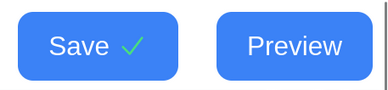
\includegraphics[width=0.4\textwidth]{pics/toolbar02.png}
    \caption{Save and Preview Buttons in Toolbar}
    \label{fig:toolbar-save-preview}
\end{figure}

\newpage

\begin{lstlisting}[language=TypeScript, caption=Saving and Previewing, label=lst:toolbar-save-preview]
<button className={SgButtonType.primarySmall} onClick={() => {
    seatgenApiClient.api.saveSeats(context.seats.map((s) => ({
        id: s.id,
        x: s.position.lat,
        y: s.position.lng,
        categoryId: s.category?.id
    })))
    .then(context.updateSaveIndex);
}} disabled={isSaveLoading}>
    {isSaveLoading ? <Spinner size={4} /> : <span>Save</span>}
</button>

<button className={SgButtonType.primarySmall} onClick={() => {
    props.setEditable(false);
    setSelectedTool(null);
}}>
    Preview
</button>
\end{lstlisting}

This save and preview mechanism shown in Listing \ref{lst:toolbar-save-preview} works as follows:
\begin{itemize}
    \item The \texttt{Save} button persists all seat and standing area modifications to the backend.
    \item A checkmark icon confirms successful saving, while a warning icon indicates unsaved changes.
    \item The \texttt{Preview} button switches the interface to a non-editable mode.
\end{itemize}

The toolbar plays a critical role in SeatGen by providing an accessible interface for stadium layout editing. It includes:
\begin{itemize}
    \item \textbf{Interactive Tool Selection:} Enables switching between different seat and area modification tools.
    \item \textbf{Map Naming:} Allows users to rename and organize stadium layouts.
    \item \textbf{Save and Preview Mechanism:} Ensures data integrity and view-only mode.
\end{itemize}

By offering an efficient and intuitive interface, the toolbar enhances the overall usability of SeatGen.
